\documentclass[]{article}

\usepackage{caption,subcaption,graphicx,float,url,amsmath,amssymb,amsthm,tocloft,cancel,mathrsfs}
\usepackage[toc,nonumberlist]{glossaries}
\usepackage{glossaries-extra,thmtools,gensymb,braket,bm,tensor}
\usepackage[toc,page]{appendix}
\usepackage[T1]{fontenc}
\usepackage[utf8]{inputenc}
\usepackage[toc,page]{appendix}
\newcommand\numberthis{\addtocounter{equation}{1}\tag{\theequation}}
\newcommand{\Lagr}{\mathscr{L}}
\newtheorem{thm}{Theorem}
\newtheorem{defn}[thm]{Definition}
\newtheorem{cor}[thm]{Corollary}
\newtheorem{lemma}[thm]{Lemma}
\graphicspath{{figs/}}
\widowpenalty10000
\clubpenalty10000
\setcounter{tocdepth}{2}

%opening
\title{Theoretical Minimum\\Cosmology}
\author{Simon Crase (compiler)\\simon@greenweaves.nz}

\begin{document}

\maketitle

\begin{abstract}
	These are my notes for the \emph{Cosmology}\cite{susskind2013cosmology} lectures from Leonard Susskind's \emph{Theoretical Minimum} series\cite{susskind2007theoretical}. 
	
	Disclaimer: I have created these notes as an aide-m\'emoire for my own use; if you find them useful, you are welcome, but I'd appreciate hearing from you. They are not intended 
	as a substitute for listening to the lectures. The intellectual property for all material derived from the lectures belongs, of course, to Professor Susskind; any mistakes, however, are my own.
	
	The notes were created using TexStudio\cite{TexStudio}, which I recommend for compiling them to a PDF, and the bibliography was created using JabRef\cite{Jabref}.
\end{abstract}

\tableofcontents
\listoffigures
\listoftables
\listoftheorems

\section{The expanding (Newtonian) universe}

Cosmology as a science dates back to the discovery of the microwave radiation from the Big Bang in the 1960s. Before that Cosmology was more like natural science--classifying oddities. Thinking of the universe as a physical system, as a system to study mathematically, with a set of physical principles and a set of equations is relatively new.

We will study the universe as a physical system.

First observation: the universe is isotropic. So it should be homogeneous.

There are around $10^{11}$ galaxies within view of Earth.

\subsection{How would Newton have handled expanding universe?}

\begin{figure}[H]
	\begin{center}
		\caption{We start by introducing a set of coordinates.}
		\begin{subfigure}[t]{0.45\textwidth}
			\caption{Chose grid so that galaxies are at grid points, so grid moves with galaxies. Galaxies move coherently (from observation).}\label{fig:cosmo-1-grid}
			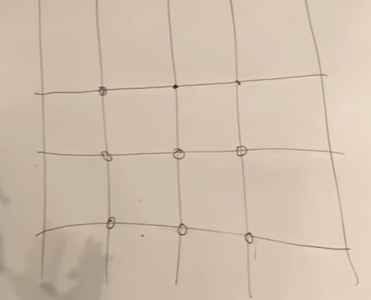
\includegraphics[width=0.8\textwidth]{cosmo-1-grid}
		\end{subfigure}
		\;
		\begin{subfigure}[t]{0.45\textwidth}
			\caption{Define distance: $D_{ab}=a(t) \Delta x_{ab}$, where scale parameter $a$ may or may not be a constant.}\label{fig:cosmo-1-distance}
			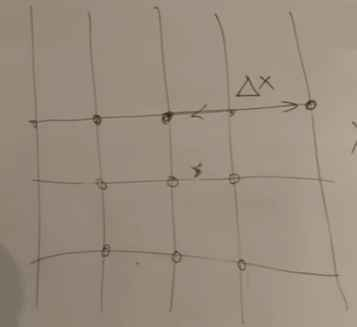
\includegraphics[width=0.8\textwidth]{cosmo-1-distance}
		\end{subfigure}
	\end{center}
\end{figure}
 
 A more general formula for distance between two galaxies $a$ and $b$ is:
 
 \begin{align*}
 	D_{ab}=&a(t) \sqrt{\Delta_{ab} x^2 + \Delta_{ab} y^2 + \Delta_{ab} z^2} \text{, now calculate velocity}\\
 	V_{ab}=&\dot{a} \Delta x_{ab} \text{, neglecting $y$ and $z$}\\
 	\frac{V_{ab}}{D_{ab}} =& \frac{\dot{a}}{a} \text{, independent of choice of galaxies!}\\
 	=& H \text{, Hubble constant at a given time.}\\
 	V =& H D \text{, Hubble's Law.}
\end{align*}
 
\subsection{How much mass is in $\Delta x \Delta y \Delta z$?}

Let $M$ denote the mass within $\Delta x \Delta y \Delta z$: $M = \nu \Delta x \Delta y \Delta z$, and $V$ denote the volume.

\begin{align*}
	V =& a^3 \Delta x \Delta y \Delta z\\
	M =& \nu \Delta x \Delta y \Delta z \text{, constant}\\
	\rho =& \frac{\nu}{a^3}
\end{align*}




\url{https://youtu.be/P-medYaqVak?t=1170}

\section{Matter and radiation dominated universes}
\section{Geometries of space: flat, spherical, hyperbolic}
\section{Cosmological Thermodynamics}
\section{Vacuum energy}
\section{Dark matter and allocation of energy density}
\section{Temperature History of the Universe}
\section{Baryogenesis}
\section{Inflation}
\section{Inhomogeneities and quantum fluctuations}


\bibliographystyle{unsrt}
\addcontentsline{toc}{section}{Bibliography}
\raggedright
\bibliography{tm}

\end{document}
